\documentclass[a4paper,12pt,catalan]{article}

\usepackage{mathpazo}
\usepackage[scaled=1.03,varqu]{zi4}
%\usepackage[scaled=0.92]{luximono}
\usepackage[T1]{fontenc}
\usepackage[utf8]{inputenc}
\usepackage{babel}

% Format
\usepackage{geometry}
\geometry{verbose,tmargin=3cm,bmargin=3cm,lmargin=3cm,rmargin=3cm}
\usepackage{setspace}
\onehalfspacing

% Referències
\usepackage[unicode=true,
  bookmarks=true,bookmarksnumbered=false,bookmarksopen=false,
  breaklinks=false,pdfborder={0 0 0},backref=false,colorlinks=false]
    {hyperref}
\hypersetup{pdfauthor={Gispert Sánchez, Francesc; Rodríguez Guasch, Sergio}}
\renewcommand{\figureautorefname}{Figura}
\renewcommand{\sectionautorefname}{Secció}
\renewcommand{\subsectionautorefname}{Secció}
\usepackage[style=numeric,sorting=nty,date=year,backend=biber]{biblatex}
\bibliography{bibliografia-informe}
\DeclareNameAlias{default}{last-first}
\setcounter{biburllcpenalty}{7000}
\setcounter{biburlucpenalty}{8000}

% Gràfics
\usepackage{graphicx}
\usepackage{pgfplots}
\pgfplotsset{compat=1.10}
\usepackage{standalone}
\usepackage{tikz}
\usetikzlibrary{circuits.logic.US}
\makeatletter
% Data Flip Flip (DFF) shape
\pgfdeclareshape{dff}{
  % The 'minimum width' and 'minimum height' keys, not the content, determine
  % the size
  \savedanchor\northeast{%
    \pgfmathsetlength\pgf@x{\pgfshapeminwidth}%
    \pgfmathsetlength\pgf@y{\pgfshapeminheight}%
    \pgf@x=0.5\pgf@x
    \pgf@y=0.5\pgf@y
  }
  % This is redundant, but makes some things easier:
  \savedanchor\southwest{%
    \pgfmathsetlength\pgf@x{\pgfshapeminwidth}%
    \pgfmathsetlength\pgf@y{\pgfshapeminheight}%
    \pgf@x=-0.5\pgf@x
    \pgf@y=-0.5\pgf@y
  }
  % Inherit from rectangle
  \inheritanchorborder[from=rectangle]

  % Define same anchor a normal rectangle has
  \anchor{center}{\pgfpointorigin}
  \anchor{north}{\northeast \pgf@x=0pt}
  \anchor{east}{\northeast \pgf@y=0pt}
  \anchor{south}{\southwest \pgf@x=0pt}
  \anchor{west}{\southwest \pgf@y=0pt}
  \anchor{north east}{\northeast}
  \anchor{north west}{\northeast \pgf@x=-\pgf@x}
  \anchor{south west}{\southwest}
  \anchor{south east}{\southwest \pgf@x=-\pgf@x}
  \anchor{text}{
    \pgfpointorigin
    \advance\pgf@x by -.5\wd\pgfnodeparttextbox%
    \advance\pgf@y by -.5\ht\pgfnodeparttextbox%
    \advance\pgf@y by +.5\dp\pgfnodeparttextbox%
  }

  % Define anchors for signal ports
  \anchor{D}{
    \pgf@process{\northeast}%
    \pgf@x=-1\pgf@x%
    \pgf@y=.5\pgf@y%
  }
  \anchor{CLK}{
    \pgf@process{\northeast}%
    \pgf@x=-1\pgf@x%
    \pgf@y=-.66666\pgf@y%
  }
  \anchor{Q}{
    \pgf@process{\northeast}%
    \pgf@y=0pt%
  }
  \anchor{R}{
    \pgf@process{\northeast}%
    \pgf@x=0pt%
  }
  \anchor{E}{
    \pgf@process{\northeast}%
    \pgf@x=0pt%
    \pgf@y=-\pgf@y%
  }
  % Draw the rectangle box and the port labels
  \backgroundpath{
    % Rectangle box
    \pgfpathrectanglecorners{\southwest}{\northeast}
    % Angle (>) for clock input
    \pgf@anchor@dff@CLK
    \pgf@xa=\pgf@x \pgf@ya=\pgf@y
    \pgf@xb=\pgf@x \pgf@yb=\pgf@y
    \pgf@xc=\pgf@x \pgf@yc=\pgf@y
    \pgfmathsetlength\pgf@x{1.6ex} % size depends on font size
    \advance\pgf@ya by \pgf@x
    \advance\pgf@xb by \pgf@x
    \advance\pgf@yc by -\pgf@x
    \pgfpathmoveto{\pgfpoint{\pgf@xa}{\pgf@ya}}
    \pgfpathlineto{\pgfpoint{\pgf@xb}{\pgf@yb}}
    \pgfpathlineto{\pgfpoint{\pgf@xc}{\pgf@yc}}
    \pgfclosepath

    % Draw port labels
    \begingroup
    \tikzset{flip flop/port labels} % Use font from this style
    \tikz@textfont

    \pgf@anchor@dff@D
    \pgftext[left,base,at={\pgfpoint{\pgf@x}{\pgf@y}},x=\pgfshapeinnerxsep]{\raisebox{-0.75ex}{D}}

    \pgf@anchor@dff@Q
    \pgftext[right,base,at={\pgfpoint{\pgf@x}{\pgf@y}},x=-\pgfshapeinnerxsep]{\raisebox{-.75ex}{Q}}

    \pgf@anchor@dff@R
    \pgftext[top,at={\pgfpoint{\pgf@x}{\pgf@y}},y=-\pgfshapeinnerysep]{R}

    \pgf@anchor@dff@E
    \pgftext[bottom,at={\pgfpoint{\pgf@x}{\pgf@y}},y=\pgfshapeinnerysep]{E}
    \endgroup
  }
}
% Key to add font macros to the current font
\tikzset{add font/.code={\expandafter\def\expandafter\tikz@textfont\expandafter{\tikz@textfont#1}}} 
% Define default style for this node
\tikzset{flip flop/port labels/.style={font=\rmfamily\scriptsize}}
\tikzset{every dff node/.style={draw,minimum width=2cm,minimum 
height=2.828427125cm,inner sep=1mm,outer sep=0pt,cap=round,add 
font=\rmfamily}}
% Data Flip Flip (DFF) shape
\pgfdeclareshape{dffne}{
  % The 'minimum width' and 'minimum height' keys, not the content, determine
  % the size
  \savedanchor\northeast{%
    \pgfmathsetlength\pgf@x{\pgfshapeminwidth}%
    \pgfmathsetlength\pgf@y{\pgfshapeminheight}%
    \pgf@x=0.5\pgf@x
    \pgf@y=0.5\pgf@y
  }
  % This is redundant, but makes some things easier:
  \savedanchor\southwest{%
    \pgfmathsetlength\pgf@x{\pgfshapeminwidth}%
    \pgfmathsetlength\pgf@y{\pgfshapeminheight}%
    \pgf@x=-0.5\pgf@x
    \pgf@y=-0.5\pgf@y
  }
  % Inherit from rectangle
  \inheritanchorborder[from=rectangle]

  % Define same anchor a normal rectangle has
  \anchor{center}{\pgfpointorigin}
  \anchor{north}{\northeast \pgf@x=0pt}
  \anchor{east}{\northeast \pgf@y=0pt}
  \anchor{south}{\southwest \pgf@x=0pt}
  \anchor{west}{\southwest \pgf@y=0pt}
  \anchor{north east}{\northeast}
  \anchor{north west}{\northeast \pgf@x=-\pgf@x}
  \anchor{south west}{\southwest}
  \anchor{south east}{\southwest \pgf@x=-\pgf@x}
  \anchor{text}{
    \pgfpointorigin
    \advance\pgf@x by -.5\wd\pgfnodeparttextbox%
    \advance\pgf@y by -.5\ht\pgfnodeparttextbox%
    \advance\pgf@y by +.5\dp\pgfnodeparttextbox%
  }

  % Define anchors for signal ports
  \anchor{D}{
    \pgf@process{\northeast}%
    \pgf@x=-1\pgf@x%
    \pgf@y=.5\pgf@y%
  }
  \anchor{CLK}{
    \pgf@process{\northeast}%
    \pgf@x=-1\pgf@x%
    \pgf@y=-.5\pgf@y%
  }
  \anchor{Q}{
    \pgf@process{\northeast}%
    \pgf@y=0pt%
  }
  \anchor{R}{
    \pgf@process{\northeast}%
    \pgf@x=0pt%
  }
  % Draw the rectangle box and the port labels
  \backgroundpath{
    % Rectangle box
    \pgfpathrectanglecorners{\southwest}{\northeast}
    % Angle (>) for clock input
    \pgf@anchor@dffne@CLK
    \pgf@xa=\pgf@x \pgf@ya=\pgf@y
    \pgf@xb=\pgf@x \pgf@yb=\pgf@y
    \pgf@xc=\pgf@x \pgf@yc=\pgf@y
    \pgfmathsetlength\pgf@x{1.6ex} % size depends on font size
    \advance\pgf@ya by \pgf@x
    \advance\pgf@xb by \pgf@x
    \advance\pgf@yc by -\pgf@x
    \pgfpathmoveto{\pgfpoint{\pgf@xa}{\pgf@ya}}
    \pgfpathlineto{\pgfpoint{\pgf@xb}{\pgf@yb}}
    \pgfpathlineto{\pgfpoint{\pgf@xc}{\pgf@yc}}
    \pgfclosepath

    % Draw port labels
    \begingroup
    \tikzset{flip flop/port labels} % Use font from this style
    \tikz@textfont

    \pgf@anchor@dffne@D
    \pgftext[left,base,at={\pgfpoint{\pgf@x}{\pgf@y}},x=\pgfshapeinnerxsep]{\raisebox{-0.75ex}{D}}

    \pgf@anchor@dffne@Q
    \pgftext[right,base,at={\pgfpoint{\pgf@x}{\pgf@y}},x=-\pgfshapeinnerxsep]{\raisebox{-.75ex}{Q}}

    \pgf@anchor@dffne@R
    \pgftext[top,at={\pgfpoint{\pgf@x}{\pgf@y}},y=-\pgfshapeinnerysep]{R}
    \endgroup
  }
}
% Define default style for this node
%\tikzset{flip flop/port labels/.style={font=\rmfamily\scriptsize}}
\tikzset{every dffne node/.style={draw,minimum width=2cm,minimum 
height=2cm,inner sep=1mm,outer sep=0pt,cap=round,add 
font=\rmfamily}}
\makeatother


% Matemàtiques 
\usepackage{mathtools}

% Codi
\usepackage{xcolor}
\usepackage{listings}
\lstloadlanguages{Java}
\lstset{%
  % backgroundcolor=\color{yellow!10},%
  aboveskip=20pt,%
  % belowskip=20pt,%
  captionpos=b,%
  frame=single,%
  basicstyle=\small\ttfamily,%
  numbers=left,%
  numberstyle=\scriptsize,%
  stepnumber=1,%
  numbersep=5pt,%
  extendedchars=true,%
  showspaces=false,%
  showtabs=false,%
  breaklines=true,%
  columns=fullflexible,%
  escapeinside={(*@}{@*)}%
}
\lstdefinestyle{antlr-gram}{%
  moredelim=[s][\color{green!70!black}]{'}{'},%
  moredelim=*[s][\color{black}]{\{}{\}},%
  moredelim=*[s][\color{black}]{[}{]},%
  commentstyle={\color{gray}},%
  morecomment=[l]{//},%
  morecomment=[s]{/*}{*/},%
  keywordstyle={\color{black}},%
  emph={grammar,hw_compilation,options,tokens,@header,@lexer,header},%
  emphstyle={\color{black}\bfseries},%
  identifierstyle=\idstyle%
}
\lstdefinestyle{hw-comp}{%
  morekeywords={VECTOR_SIZE,IF,THEN,ELSE,FI,WHILE,DO,ELIHW,FUNC,CNUF,ARG,GRA,VAR,RAV},%
  keywordstyle=\bfseries\color{blue},%
  alsoletter={0,1,2,3,4,5,6,7,8,9},
  emph={0,1,2,3,4,5,6,7,8,9,0x,0b},%
  emphstyle={\color{red}},%
  identifierstyle=\numstyle%
}
\lstdefinestyle{java}{%
  language=Java,%
  keywordstyle=\bfseries\color{blue},%
  commentstyle=\color{gray},%
  stringstyle=\color{red},%
  emphstyle=\bfseries\color{violet}%
}
\makeatletter
\newcommand*\idstyle{%
  \expandafter\id@style\the\lst@token\relax%
}
\def\id@style#1#2\relax{%
  \ifcat#1\relax\else%
    \ifnum`#1=\uccode`#1%
      \color{blue}%
    \else%
      \ifnum`#1=\lccode`#1%
        \color{violet}%
      \fi%
    \fi%
  \fi%
}
\newcommand*\numstyle{%
  \expandafter\num@style\the\lst@token\relax%
}
\def\rednum#1{%
  \if!\ifnum9<1#1!\else_\fi
    \color{red}\else\relax\fi
}
\def\num@style#1#2\relax{%
  \ifcat#1\relax\else%
    \rednum#1%
  \fi%
}
\makeatother
\renewcommand*\lstlistingname{Fragment de codi}

% Altres paquets
\usepackage[binary-units]{siunitx}  % Unitats del SI
\usepackage{mleftright}  % Arregla problema d'espais abans de parèntesis
\let\left\mleft
\let\right\mright


\begin{document}

\title{Compiladors\\ Documentació de HW--Compilation}  

\author{Gispert Sánchez, Francesc-Xavier \and Rodríguez Guasch, Sergio}

\maketitle

\noindent \rule[0.5ex]{1\columnwidth}{1pt}

\tableofcontents

\clearpage

%%%%%%%%%%%%%%%%%%%%%%%%%%%%%%%%%%%%%%%%%%%%%%%%%%%%%%%%%%%%%%%%%%%%%%%%%%%%%%%


\section{Introducció}

Tradicionalment, aprenem de forma independent i aïllada el funcionament del 
\textit{hardware} dels computadors i la programació mitjançant 
\textit{software}. Malgrat les capes d'abstracció que afegim entremig, però, 
és clar que és tècnicament possible, per a cada programa que puguem expressar 
mitjançant qualsevol llenguatge de programació, dissenyar un circuit lògic que 
l'executi.

Aquest projecte té com a objectiu fonamental mostrar que, a més, es pot fer 
aquest pas d'un programa expressat en un llenguatge de programació 
convencional a un circuit digital equivalent de forma automàtica. 

A tal efecte, dissenyem un llenguatge de programació molt simple de capacitats 
reduïdes però amb algunes de les estructures de seqüenciació més habituals i 
construirem un traductor que, a partir dels programes especificats en aquest 
llenguatge, generi automàticament els circuits corresponents. En particular, 
aquest llenguatge de programació tractarà amb vectors de bits d'una mida 
fixada per a cada programa (que, llavors, el programador pot interpretar com a 
nombres enters, per exemple) i disposarà de sentències condicionals i 
repetitives, així com d'un sistema de funcions i crides a aquestes. Una de 
les principals limitacions d'aquest llenguatge, però, serà la falta de memòria 
(cosa que, d'altra banda, facilitarà la simulació dels programes en circuits). 

Tanmateix, l'interès d'aquest projecte no deixa de ser merament acadèmic, ja 
que els circuits generats no són en general òptims (ni pretenen ser-ho) i, per 
tant, amb programes d'una complexitat mitjana ja és possible tenir una 
explosió de portes lògiques que en faci infactible la implementació a la 
pràctica. Per aquest motiu, un llenguatge limitat com el descrit és suficient 
per exemplificar la traducció automàtica de programes a circuits.



\clearpage


\section{Especificació del llenguatge}

El llenguatge que dissenyem serà, en principi, molt simple i limitat. Això ens 
permetrà concentra-nos en la part més interessant del projecte, que és la de 
traducció de \textit{software} a \textit{hardware}. De totes maneres, vegem 
a continuació les principals característiques del llenguatge.

Al principi de cada programa, el programador ha de fixar la mida dels vectors 
de bits que s'utilitzaran. Llavors, la sintaxi del llenguatge permet aplicar 
operacions molt senzilles sobre aquests vectors de bits: sumes i restes 
(interpretant els vectors com a enters codificats en complement a dos); 
conjuncions, disjuncions i negacions bit a bit; conjuncions, disjuncions i 
negacions lògiques (entenent que tot vector diferent de zero codifica el valor 
cert), i comparacions d'igualtat i desigualtat. La precedència dels operadors 
és la mateixa que a \texttt{C}.

Un programa està format per una o més funcions, una de les quals s'ha 
d'anomenar \texttt{main}: aquesta serà, com el seu nom indica, el punt 
d'entrada a l'execució. Cadascuna d'aquestes funcions pot rebre alguns 
arguments i ha de retornar exactament un vector de bits com a sortida. A més, 
les variables utilitzades per una funció han d'haver estat declarades al 
principi d'aquesta (això facilitarà el procés de traducció, ja que, en traduir 
el programa a un circuit, cada variable correspondrà a un registre), i una 
funció només té accés a aquestes variables, així com als seus paràmetres. Una 
variable especial amb el mateix nom que la funció emmagatzemarà el valor de 
retorn: aquesta s'haurà d'assignar a l'última línia del cos de la funció (per 
tal de facilitar l'anàlisi semàntica dels programes). 

Les instruccions bàsiques del llenguatge seran assignacions i sentències de 
control de flux. En particular, el llenguatge disposa d'una estructura 
condicional (\textit{if-then-else}) i una estructura repetitiva 
(\textit{while}). 

A partir de les operacions mencionades prèviament i l'ús de literals 
(especificats en bases binària, decimal o hexadecimal), variables i crides a 
funcions, es construeixen les expressions bàsiques del llenguatge.

Com ja s'ha explicat, aquest llenguatge no simula una memòria i tampoc permet 
recursivitat. Així, totes les variables a utilitzar han d'haver estat 
prèviament definides pel programador estàticament. Per tant, l'expressivitat 
del llenguatge és força limitada (tot i que és més que suficient per a 
l'objectiu d'aquest projecte).

Finalment, segueixen alguns exemples d'ús del llenguatge. En particular, al 
\autoref{lst:ex-enters} es mostren alguns algorismes elementals utilitzats en 
teoria de nombres, mentre que al \autoref{lst:ex-xifrat} es mostra una 
estratègia molt simple per xifrar i desxifrar blocs de dades. En aquests 
exemples es poden observar les construccions bàsiques que permet el llenguatge.

\lstinputlisting%
  [caption={Exemple d'ús per funcions en enters.},style=hw-comp,label={lst:ex-enters}]%
  {../examples/number_theory.hwc}

\lstinputlisting%
  [caption={Exemple d'ús en un mètode de xifrat.},style=hw-comp,label={lst:ex-xifrat}]%
  {../examples/tea.hwc}




\clearpage


\section{Mòduls del projecte}

Dividirem el projecte essencialment en tres mòduls, la funció dels quals es 
descriu breument a continuació.

\subsection{Analitzador lèxico-sintàctic}
Com a gairebé qualsevol llenguatge, a la primera part del \textit{pipeline} té 
lloc l'anàlisi lèxica i sintàctica. Aquest mòdul, generat automàticament amb 
\texttt{ANTLR}, serà el que rebi un fitxer de codi com a entrada i retorni, si 
el codi resulta ser correcte a nivell sintàctic, el seu AST corresponent. En 
aquesta secció considerarem que un codi és correcte si aquest es pot 
obtenir com a resultat de les regles de producció de la gramàtica adjunta al 
\autoref{lst:gramatica}.

\subsection{Analitzador semàntic}
Un cop generat l'arbre sintàctic, cal realitzar unes certes comprovacions que 
assegurin que el programa presentat inicialment és totalment correcte i 
traduïble. Al marge de les condicions habituals presents a la majoria de 
llenguatges, cal assegurar-se també que no existeix cap successió de crides a 
funcions que provoquin un cicle. Amb aquesta finalitat, el que es farà serà 
generar un graf dirigit on cada funció serà un node i, donats dos nodes \(f\) 
i \(g\), nomès existirà un arc \((f,g)\) si \(f\), en algun punt (o en 
diversos) del seu codi, crida a \(g\). Considerarem que un programa és correcte 
respecte de les crides quan el graf generat sigui acíclic. Aquesta restricció 
imposada elimina, per tant, l'existència de qualsevol tipus de recursivitat 
(però no les crides multinivell). L'arbre sintàctic generat a la primera fase 
i el graf de crides derivat d'aquest seran l'entrada que rebrà el mòdul de la 
següent (i última) fase.

\subsection{Generador de \textit{hardware}}
Finalment, un cop comprovada la consistència sintàctica i semàntica, es 
realitza la traducció a \textit{hardware} del programa que s'ha rebut 
inicialment com a entrada. Aquesta traducció consisteix a convertir el codi 
en \texttt{Verilog} sintetitzable el qual descrigui un circuit que implementi 
el programa inicial proposat. De manera similar a com fan molts llenguatges 
compilats, aquesta traducció consistirà en l'aplicació sistemàtica de regles 
predefinides que indiquen com s'ha d'implementar cadascuna de les construccions 
del llenguatge. Cal especificar que, en aquesta fase, el graf de crides 
prèviament generat per l'analitzador semàntic és especialment útil, ja que 
aquest ens indicarà quins mòduls de funcions s'han d'interconnectar.



\clearpage

\section{Operacions sobre l'arbre sintàctic} \label{sec:graf}

En aquesta secció, s'ofereix una explicació més detallada de la obtenció de 
certa informació intermèdia que s'ha encabit en el mòdul d'anàlisi semàntica.

Cal recordar que aquesta part és la que s'executa immediatament desprès de 
l'anàlisi lèxico-sintàctica (si aquesta ha resultat reeixida). En aquesta part 
es comprova que les restriccions més típiques de llenguatges similars a 
l'emprat se satisfacin (per exemple, que no s'utilitzin variables no 
declarades, que no es redeclarin variables i altres normes similars). Donades 
les particularitats del llenguatge, també cal comprovar que cap de totes les 
possibles successions de crides que poden tenir lloc al programa desemboquin 
en recursivitat.

Aquesta part d'anàlisi semàntica també s'encarrega de realitzar uns certs 
càlculs necessaris per a la part posterior, la qual s'encarrega de traduir 
finalment el programa donat en un circuit descrit en \texttt{Verilog} 
sintetitzable. També es construeix, de forma simultània a les comprovacions 
semàntiques i els càlculs anteriorment esmentats, un graf $G$ i el seu 
transposat $G^{T}$, el qual conté com a nodes les funcions del programa. Una 
aresta $(f,g)$ és present a $G$ si $f$ crida a $g$ en algun punt del programa 
(o en diversos).

La tasca d'anàlisi semàntica s'ha dividit en tres etapes: preprocessament, 
recorregut explícit de l'AST generat al mòdul anterior i comprovació de 
funcions no utilitzades i recursivitat. Cal remarcar que, al disseny presentat,
les comprovacions semàntiques i els càlculs necessaris per a la següent fase 
es duen a terme de forma simultània, ja que aquests dos procediments no 
presenten cap mena de dependència entre ells.


\subsection{Preprocessament}

És útil obtenir certa informació prèviament al recorregut de l'AST obtingut a 
la fase anterior. Aquesta tasca consisteix a obtenir els noms i les referències
als nodes de les funcions declarades al programa. Amb aquestes dades es pot 
comprovar que cap nom de funció es declari més d'una vegada i que hi hagi una 
funció principal definida. Aquestes dades també permeten inicialitzar 
estructures de dades auxiliars, com ara els dos grafs de crides (els 
quals consistiran, després d'aquesta fase, en grafs amb tants nodes com 
funcions hi hagi i sense cap aresta). Si es troba qualsevol error, l'execució 
s'avorta en aquesta fase i no es passa a la següent.


\subsection{Recorregut de l'AST}

En aquesta etapa de l'anàlisi es recorre l'arbre sintàctic pròpiament dit. 
Donades les necessitats específiques del llenguatge, la classe que representa 
l'arbre sintàctic no és la pròpia d'\texttt{ANTLR}, sinó una extensió 
d'aquesta. Concretament, s'ha estès per permetre que cada node contingui 
informació sobre quina és la seva funció d'origen. Pels nodes que representen 
una crida a funció també es guarda un enter que indica quin número de crida 
representen dins la seva funció origen (és a dir, es tracta d'identificadors 
de les crides: si l'identificador d'una crida és 5, vol dir que aquest node 
representa la cinquena crida a funció que es pot trobar al codi de la seva 
funció origen). Quelcom similar es fa per a les assignacions.

L'estratègia de recorregut és senzilla: s'obté el node que representa la 
funció principal i es recorre tot l'arbre accessible des d'aquest. Durant el 
recorregut, es pot estar en diferents estats segons els tipus de node: funció, 
llista d'instruccions, instrucció i expressió. A cada estat es comproven 
diverses restriccions semàntiques i es construeixen diferents parts de les 
estructures de dades auxiliars anteriorment comentades.

En els nodes que representen funcions es comprova, en primer lloc, que el node 
en qüestió no hagi estat processat prèviament. Tot seguit, es comprova que els 
noms de les variables i paràmetres definits siguin consistents (tant entre 
ells com amb els noms d'altres funcions). Per consistència hem d'entendre que 
no hi hagi dos elements amb el mateix nom. Aprofitem per recordar que l'àmbit 
de visibilitat pel que fa a variables i paràmetres és únicament local i que, 
per tant, dues funcions poden tenir variables i paràmetres amb els mateixos 
noms sense cap problema. Si es troba algun error en aquesta part, s'avorta 
l'anàlisi sense passar a la següent fase. També s'aprofita per a inicialitzar 
localment unes estructures de dades que mantenen el comptatge d'assignacions 
realitzades a les variables o paràmetres d'aquesta funció, les quals seran 
necessàries per a poder assignar l'identificador d'assignacions anteriorment 
esmentat. Finalment, es comprova que l'última instrucció contingui una 
assignació la part esquerra de la qual sigui el propi nom de la funció, ja que 
això, en aquest llenguatge, es considera el valor de retorn. Donat que no 
existeixen efectes laterals, es pot considerar un error el fet de tenir una 
funció sense un valor de retorn correctament definit. Si totes les 
comprovacions han resultat correctes, es procedeix a recórrer la llista 
d'instruccions, la qual representa el codi de la funció. En l'anàlisi del cos 
de la funció, doncs, es manté un registre del nom de la funció d'origen i els 
noms visibles (arguments i variables).

Per a les llistes d'instruccions, simplement es processen tots els fills (els 
quals seran instruccions) de manera successiva, parant si algun d'aquests 
provoca un error.

Els nodes que representen instruccions es tracten per casos (un cas per tipus 
d'instrucció). Els casos possibles són: assignació, condicional (\textit{if}) i 
bucle (\textit{while}).

Pel cas de l'assignació, es comprova, en primer lloc, que l'identificador de 
la part esquerra sigui, en efecte, una variable visible dins l'àmbit de la 
funció a la qual s'està. Tot seguit, s'assigna un identificador d'assignació 
al node en qüestió i s'actualitza el comptatge d'aquestes. Finalment, si no hi 
ha hagut errors, es recorre l'expressió que correspon a la part dreta de 
l'assignació.

En els condicionals, es comença recorrent l'expressió que correspon a la 
condició. Si no hi ha hagut cap error, es recorre la llista d'instruccions del 
\textit{then}. Si no hi ha hagut cap error, es comprova si existeix un últim 
node del tipus llista d'instruccions (el qual representaria l'\textit{else}); 
en cas afirmatiu, també es recorre. Els bucles es processen de forma similar, 
obviant la part de l'\textit{else}.

L'últim cas a tenir en compte són els nodes que corresponen a les expressions. 
Aquests nodes també es tracten diferent segons de quin tipus siguin. Aquí 
podem distingir els següents casos: identificador, literal enter, crida a 
funció i operadors aritmètics.

Pel cas de l'identificador, simplement es comprova que aquest faci referència 
a algun dels noms de variables o paràmetres visibles en l'àmbit en qüestió.

Els literals s'ignoren i no es fa res amb ells. Això es degut a què, en 
aquesta part, no es necessita comprovar res dels seus valors: els problemes 
que aquests podrien donar en temes de correcció es detecten a la fase 
d'anàlisi sintàctica, la qual és anterior a aquesta.

Les crides a funcions es tracten com segueix: es comprova primer que la funció 
cridada existeix i que l'aritat proposada (el nombre d'arguments) coincideix 
amb l'aritat real d'aquesta. També es recorren les expressions que representen 
els paràmetres. Finalment, es recorre la funció que s'està cridant. 
Addicionalment, s'afegeixen les arestes corresponents als dos grafs de crides.

Finalment, pels operadors aritmètics o lògics es comproven recursivament les 
expressions que es tenen com a operands.


\subsection{Comprovació de recursivitat}

Un cop acabat el processament descrit a la secció anterior, es procedeix a 
comprovar que no existeixi cap successió de crides que desemboqui en 
recursivitat, ja sigui directa o indirecta. Per això, es mira que cap funció 
no es cridi a si mateixa i que el graf dirigit de crides $G$ generat no 
contingui cap component fortament connexa de més d'un vèrtex. Donat que 
l'algorisme fet servir per aquesta detecció és constructiu, es pot donar com a 
missatge d'error el conjunt (o conjunts) exacte de funcions que creen 
recursivitat. Com a efecte lateral de l'execució d'aquest algorisme, també 
s'obté una col·lecció de noms de funcions, els quals representen les funcions 
que són potencialment utilitzades en l'execució del programa. Això és 
especialment útil per a la següent fase, ja que permet fer una traducció 
selectiva, podent resultar en programes més petits que els que s'obtindrien si 
la traducció fos del tot sistemàtica. Aquesta col·lecció també es fa servir per 
emetre avisos de codi no emprat al programa final.




\clearpage


\section{Traducció a circuits}

En aquesta secció, es descriuen les regles dissenyades per traduir de forma 
automàtica el codi del nostre llenguatge a circuits lògics (expressats en el 
llenguatge \texttt{Verilog}). Les idees fonamentals estan basades en 
l'exposició de \cite{wirth1998hardware} (tot i que s'han ampliat per permetre 
construccions diferents de les mostrades en l'article citat).

Les explicacions d'aquesta secció es basen en diversos diagrames de circuits 
que en faciliten la comprensió. En aquests, s'ha seguit la convenció 
d'utilitzar línies fines per als cables d'un únic bit i línies més gruixudes 
per representar els busos de \(n\) bits (on \(n\) és un nombre especificat per 
l'usuari del llenguatge al principi del programa a traduir; en els subsegüents
diagrames s'utilitzarà \(n=2\) per simplicitat). A més, aquests circuits 
corresponen a l'execució d'un codi i, per tant, s'ha intentat que es 
puguin interpretar d'aquesta manera veient-los ``d'esquerra a dreta'' (en 
particular, quan apareixen diversos senyals amb el mateix nom, el senyal de 
l'esquerra correspon a l'entrada d'aquell fragment de circuit, mentre que el 
senyal de la dreta correspon a la sortida).

Els circuits s'expressen utilitzant només portes lògiques i biestables de 
dos tipus. Els del primer tipus tenen un senyal d'entrada \textsc{d}, un de 
sortida \textsc{q} i un de reinici \textsc{r}. Quan hi ha un flanc ascendent 
del rellotge es canvia el valor de \textsc{q}: si el valor de \textsc{r} és 1, 
aleshores \textsc{q} passa a valdre 0; altrament, el valor de \textsc{q} 
passa a ser el valor de \textsc{d}. Els biestables del segon tipus 
funcionen de forma similar però, a més, tenen un senyal d'activació 
\textsc{e}. Així, quan hi ha un flanc ascendent de rellotge i el valor de 
\textsc{r} és 0, només es canvia el valor de \textsc{q} pel de \textsc{d} si 
el valor de \textsc{e} és 1 (altrament, el valor de \textsc{q} roman 
inalterat). 

Per traduir un programa a \textit{hardware}, es van generant recursivament 
fragments d'un circuit lògic seguint l'estructura de l'AST que representa les 
instruccions del programa. Aquests circuits es componen de dues parts: d'una 
banda, hi ha una part principal del circuit que efectua els càlculs expressats 
en les instruccions del programa; de l'altra, hi ha una segona part igual 
d'important que controla el flux de l'execució (és a dir, activa i desactiva 
els diferents components del primer circuit per garantir que les operacions 
s'efectuen seguint l'ordre correcte). Vegem ara com es tradueixen els 
diferents tipus d'instruccions.

\begin{figure}[ht]
    \centering
    \documentclass[tikz,12pt,border=12pt]{standalone}

\usepackage{mathpazo}
\usepackage[scaled=1.03,varqu]{zi4}
\usepackage[T1]{fontenc}
\usepackage[utf8]{inputenc}
\usepackage{mathtools}
\usepackage{pgf,tikz}
\usetikzlibrary{circuits.logic.US}


\begin{document}

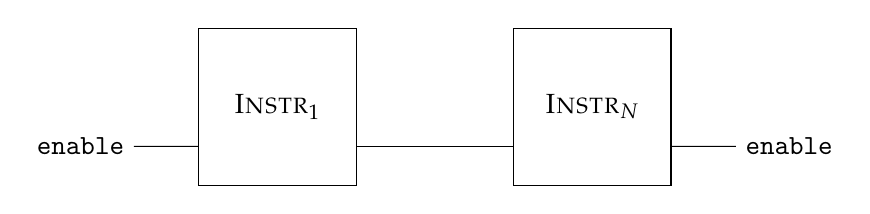
\begin{tikzpicture}[circuit logic US,%
        dot/.style    = {anchor=base,fill,circle,inner sep=1.3pt}]

\node[draw,rectangle,minimum width=2cm,minimum height=2cm] at (1,1) (i1) {$\textsc{Instr}_1$};
\node[draw,rectangle,minimum width=2cm,minimum height=2cm] at (5,1) (in) {$\textsc{Instr}_N$};
\node at (-1.5,0.5) (e_in) {\texttt{enable}};
\node at (7.5,0.5) (e_out) {\texttt{enable}};

\draw ($ (i1.east) + (0,-0.5) $) -- ($ (in.west) + (0,-0.5) $);
\draw (e_in.east) -- ($ (i1.west) + (0,-0.5) $);
\draw ($ (in.east) + (0,-0.5) $) -- (e_out.west);

\end{tikzpicture}

\end{document}




    \caption{Circuit corresponent a una llista de \(N\) instruccions (en el 
        diagrama, per simplicitat, \(N=2\)) consecutives.}
    \label{fig:instr-list}
\end{figure}

Per traduir un bloc d'instruccions consecutives, senzillament cal traduir 
cadascuna de les instruccions per separat i encadenar els senyals d'activació. 
D'aquesta manera, es fa que el senyal de sortida del circuit corresponent a la 
primera instrucció sigui el senyal d'entrada del circuit corresponent a la 
segona instrucció, i així successivament fins a l'última. La 
\autoref{fig:instr-list} mostra la forma dels circuits obtinguts d'aquesta 
forma.

\begin{figure}[ht]
    \centering
    \documentclass[tikz,12pt,border=12pt]{standalone}

\usepackage{mathpazo}
\usepackage[scaled=1.03,varqu]{zi4}
\usepackage[T1]{fontenc}
\usepackage[utf8]{inputenc}
\usepackage{mathtools}
\usepackage{pgf,tikz}
\usetikzlibrary{circuits.logic.US}


\begin{document}

\begin{tikzpicture}[circuit logic US,%
        dot/.style    = {anchor=base,fill,circle,inner sep=1.3pt}]

\node[draw,rectangle,minimum width=2cm,minimum height=2cm] at (0,1.5) (Cond) {\textsc{Cond}};
\node[dot] at (1.5,2) (aux1_cond) {};
\node[or gate,inputs=nn] at (2.5,2) (or_cond) {};
\node[dot] at (3.5,2) (aux2_cond) {};
\node[dot] at (4,1) (aux3_cond) {};
\node[and gate,inputs=nn] at (5,3) (and_enb_if) {};
\node[and gate,inputs=in] at (5,-1) (and_enb_else) {};
\node[draw,rectangle,minimum width=2cm,minimum height=2cm] at (7,3.5) (IfT) {\textsc{IfT}};
\node[draw,rectangle,minimum width=2cm,minimum height=2cm] at (7,-0.5) (ElseT) {\textsc{IfF}};
\node[or gate,inputs=nn] at (9,1) (or_enb_end) {};
\node at ($(Cond.west) + (-1.5, -0.5) $) (e_in) {\texttt{enable}};
\node at (11,1) (e_out) {\texttt{enable}}; 

\draw[very thick] ($ (Cond.east) + (0,0.5) $) -- (aux1_cond);
\draw (aux1_cond) |- (or_cond.input 1);
\draw (aux1_cond) |- (or_cond.input 2);
\draw (or_cond.output) -- (aux2_cond) |- (and_enb_if.input 1); \draw (aux2_cond) |- (and_enb_else.input 1);
\draw ($ (Cond.east) + (0,-0.5) $) -- (aux3_cond) |- (and_enb_if.input 2); \draw (aux3_cond) |- (and_enb_else.input 2);
\draw (and_enb_if.output) -- ($ (IfT.west) + (0,-0.5) $);
\draw (and_enb_else.output) -- ($ (ElseT.west) + (0,-0.5) $);
\draw ($ (IfT.east) + (0,-0.5) $) -- ++(0.3,0) |- (or_enb_end.input 1); 
\draw ($ (ElseT.east) + (0,-0.5) $) -- ++(0.3,0) |- (or_enb_end.input 2);
\draw (e_in) -- ($ (Cond.west) + (0,-0.5) $); 
\draw (or_enb_end.output) -- (e_out);

\end{tikzpicture}

\end{document}




    \caption{Circuit corresponent a una sentència condicional.}
    \label{fig:if-else}
\end{figure}

La \autoref{fig:if-else} mostra el circuit generat per a una sentència 
condicional. En qualsevol dels casos, primerament cal avaluar la condició i, 
per tant, es genera recursivament el circuit \textsc{Cond} corresponent i s'hi 
col·loca el senyal d'activació de la sentència condicional directament. Com 
que el llenguatge dissenyat treballa amb vectors de \(n\) bits fins i tot per 
a les condicions, cal utilitzar una porta \textit{or} amb entrades cadascun 
d'aquests \(n\) bits per comprovar si la condició es verifica o no (en aquest 
llenguatge, l'únic valor amb el valor lògic fals és el 0). Els dos circuits 
corresponents a les branques condicional i alternativa d'aquesta instrucció, 
\textsc{IfT} i \textsc{IfF}, també es generen recursivament i cal muntar 
un circuit d'activació que n'activi exactament un dels dos (en funció del 
valor de la condició avaluada). A més, aquests circuits s'han d'activar 
justament després que el circuit d'avaluació de la condició. Així, doncs, el 
senyal d'activació del circuit \textsc{IfT} es connecta amb el resultat d'una 
porta \textit{and} amb entrades la condició avaluada i el senyal d'activació 
de sortida de \textsc{Cond}; anàlogament, el senyal d'activació del circuit 
\textsc{IfF} es connecta amb el resultat d'una porta \textit{and} amb entrades 
la condició avaluada negada i el senyal d'activació del circuit de sortida de 
\textsc{Cond}. Finalment, el senyal d'activació resultant després d'aquesta 
instrucció s'ha d'obtenir mitjançant una porta \textit{or} amb els senyals 
d'activació que surten de \textsc{IfT} i \textsc{IfF} (o sigui, la instrucció 
s'acaba d'executar quan alguna de les dues branques condicionals finalitza la 
seva execució). En cas que no hi hagi una branca alternativa (és a dir, un 
\textit{else}), el circuit \textsc{IfF} desapareix i la resta del circuit 
queda exactament igual.

\begin{figure}[ht]
    \centering
    \documentclass[tikz,12pt,border=12pt]{standalone}

\usepackage{mathpazo}
\usepackage[scaled=1.03,varqu]{zi4}
\usepackage[T1]{fontenc}
\usepackage[utf8]{inputenc}
\usepackage{mathtools}
\usepackage{pgf,tikz}
\usetikzlibrary{circuits.logic.US}


\begin{document}

\begin{tikzpicture}[circuit logic US,%
        dot/.style    = {anchor=base,fill,circle,inner sep=1.3pt}]

\node[draw,rectangle,minimum width=2cm,minimum height=2cm] at (0,1.5) (Cond) {\textsc{Cond}};
\node[dot] at (1.5,2) (aux1_cond) {};
\node[or gate,inputs=nn] at (2.5,2) (or_cond) {};
\node[dot] at (3.5,2) (aux2_cond) {};
\node[dot] at (4,1) (aux3_cond) {};
\node[and gate,inputs=nn] at (5,3) (and_enb_if) {};
\node[and gate,inputs=in] at (5,1.1) (and_enb_else) {};
\node[draw,rectangle,minimum width=2cm,minimum height=2cm] at (7,3.5) (WhileT) {\textsc{WhileT}};
\node at (-4.5,1.1) (e_in) {\texttt{enable}};
\node[or gate,inputs=nn] at (-2,1) (or_cond_in) {};
\node at (7,1.1) (e_out) {\texttt{enable}}; 

\draw[very thick] ($ (Cond.east) + (0,0.5) $) -- (aux1_cond);
\draw (aux1_cond) |- (or_cond.input 1);
\draw (aux1_cond) |- (or_cond.input 2);
\draw (or_cond.output) |- (aux2_cond) |- (and_enb_if.input 1); \draw (aux2_cond) |- (and_enb_else.input 1);
\draw ($ (Cond.east) + (0,-0.5) $) -- (aux3_cond);
\draw (and_enb_if.output) |- ($ (WhileT.west) + (0,-0.5) $);
\draw ($ (WhileT.east) + (0,-0.5) $) -- ++(0.5,0) -- ++(0,-3) -- ++(-11.5,0) |- (or_cond_in.input 2);
\draw (aux3_cond) -- (and_enb_else.input 2); \draw (aux3_cond) |- (and_enb_if.input 2);
\draw (e_in) -- (or_cond_in.input 1);
\draw (or_cond_in.output) -- ($ (Cond.west) + (0,-0.5) $); 
\draw (and_enb_else.output) -- (e_out);

\end{tikzpicture}

\end{document}




    \caption{Circuit corresponent a una sentència repetitiva.}
    \label{fig:while}
\end{figure}

El circuit generat per a una sentència repetitiva s'il·lustra a la 
\autoref{fig:while}. El fragment \textsc{Cond} d'aquest (que correspon a 
l'avaluació de la condició) i l'activació de \textsc{WhileT} (corresponent al 
bloc d'instruccions que conforma el cos de la sentència repetitiva) en funció 
del resultat de la condició és igual que el d'una sentència condicional
(sense \textit{else}) i, per tant, n'ometem una descripció en detall. En 
aquest cas, però, el senyal d'activació per al circuit \textsc{Cond} es 
calcula de forma diferent, ja que s'ha de poder repetir després de cada 
iteració. D'una banda, aquest s'ha d'activar quan s'inicia l'execució de la 
instrucció (abans de començar cap iteració); d'altra banda, també cal activar 
l'execució de la condició just després d'executar una iteració del cos de la 
sentència repetitiva. Per tant, es col·loca una porta \textit{or} que té per 
entrades el senyal d'activació d'entrada de la instrucció i el senyal de 
sortida del circuit \textsc{WhileT} i es connecta la sortida d'aquesta porta 
al senyal d'activació d'entrada del circuit \textsc{Cond}.  

Fins al moment ja s'ha explicat el mètode seguit per a la generació dels 
circuits que controlen el flux d'execució del programa. Així, doncs, queda 
descriure els circuits que es generen per a definir les variables i les 
funcions del programa (en aquest document no s'explica com dissenyar un 
circuit per a executar les operacions aritmètiques i lògiques bàsiques, ja 
que no és l'objectiu del projecte; de fet, aquesta tasca es deixa a l'eina de 
síntesi o de simulació del circuit perquè les operacions s'expressen 
directament en la sintaxi de \texttt{Verilog}).

\begin{figure}[ht]
    \centering
    \documentclass[tikz,12pt,border=12pt]{standalone}

\usepackage{mathpazo}
\usepackage[scaled=1.03,varqu]{zi4}
\usepackage[T1]{fontenc}
\usepackage[utf8]{inputenc}
\usepackage{mathtools}
\usepackage{pgf,tikz}
\usetikzlibrary{circuits.logic.US}


%%%%%%%%%%%%%%%%%%%%%%%%%%%%%%%%%%%%%%%%%%%%%%%%%%%%%%%%%%%%%%%%%%%%%%%%%%%%%%%

\makeatletter

% Data Flip Flip (DFF) shape
\pgfdeclareshape{dff}{
  % The 'minimum width' and 'minimum height' keys, not the content, determine
  % the size
  \savedanchor\northeast{%
    \pgfmathsetlength\pgf@x{\pgfshapeminwidth}%
    \pgfmathsetlength\pgf@y{\pgfshapeminheight}%
    \pgf@x=0.5\pgf@x
    \pgf@y=0.5\pgf@y
  }
  % This is redundant, but makes some things easier:
  \savedanchor\southwest{%
    \pgfmathsetlength\pgf@x{\pgfshapeminwidth}%
    \pgfmathsetlength\pgf@y{\pgfshapeminheight}%
    \pgf@x=-0.5\pgf@x
    \pgf@y=-0.5\pgf@y
  }
  % Inherit from rectangle
  \inheritanchorborder[from=rectangle]

  % Define same anchor a normal rectangle has
  \anchor{center}{\pgfpointorigin}
  \anchor{north}{\northeast \pgf@x=0pt}
  \anchor{east}{\northeast \pgf@y=0pt}
  \anchor{south}{\southwest \pgf@x=0pt}
  \anchor{west}{\southwest \pgf@y=0pt}
  \anchor{north east}{\northeast}
  \anchor{north west}{\northeast \pgf@x=-\pgf@x}
  \anchor{south west}{\southwest}
  \anchor{south east}{\southwest \pgf@x=-\pgf@x}
  \anchor{text}{
    \pgfpointorigin
    \advance\pgf@x by -.5\wd\pgfnodeparttextbox%
    \advance\pgf@y by -.5\ht\pgfnodeparttextbox%
    \advance\pgf@y by +.5\dp\pgfnodeparttextbox%
  }

  % Define anchors for signal ports
  \anchor{D}{
    \pgf@process{\northeast}%
    \pgf@x=-1\pgf@x%
    \pgf@y=.5\pgf@y%
  }
  \anchor{CLK}{
    \pgf@process{\northeast}%
    \pgf@x=-1\pgf@x%
    \pgf@y=-.66666\pgf@y%
  }
  \anchor{Q}{
    \pgf@process{\northeast}%
    \pgf@y=0pt%
  }
  \anchor{R}{
    \pgf@process{\northeast}%
    \pgf@x=0pt%
  }
  \anchor{E}{
    \pgf@process{\northeast}%
    \pgf@x=0pt%
    \pgf@y=-\pgf@y%
  }
  % Draw the rectangle box and the port labels
  \backgroundpath{
    % Rectangle box
    \pgfpathrectanglecorners{\southwest}{\northeast}
    % Angle (>) for clock input
    \pgf@anchor@dff@CLK
    \pgf@xa=\pgf@x \pgf@ya=\pgf@y
    \pgf@xb=\pgf@x \pgf@yb=\pgf@y
    \pgf@xc=\pgf@x \pgf@yc=\pgf@y
    \pgfmathsetlength\pgf@x{1.6ex} % size depends on font size
    \advance\pgf@ya by \pgf@x
    \advance\pgf@xb by \pgf@x
    \advance\pgf@yc by -\pgf@x
    \pgfpathmoveto{\pgfpoint{\pgf@xa}{\pgf@ya}}
    \pgfpathlineto{\pgfpoint{\pgf@xb}{\pgf@yb}}
    \pgfpathlineto{\pgfpoint{\pgf@xc}{\pgf@yc}}
    \pgfclosepath

    % Draw port labels
    \begingroup
    \tikzset{flip flop/port labels} % Use font from this style
    \tikz@textfont

    \pgf@anchor@dff@D
    \pgftext[left,base,at={\pgfpoint{\pgf@x}{\pgf@y}},x=\pgfshapeinnerxsep]{\raisebox{-0.75ex}{D}}

    \pgf@anchor@dff@Q
    \pgftext[right,base,at={\pgfpoint{\pgf@x}{\pgf@y}},x=-\pgfshapeinnerxsep]{\raisebox{-.75ex}{Q}}

    \pgf@anchor@dff@R
    \pgftext[top,at={\pgfpoint{\pgf@x}{\pgf@y}},y=-\pgfshapeinnerysep]{R}

    \pgf@anchor@dff@E
    \pgftext[bottom,at={\pgfpoint{\pgf@x}{\pgf@y}},y=\pgfshapeinnerysep]{E}
    \endgroup
  }
}

% Key to add font macros to the current font
\tikzset{add font/.code={\expandafter\def\expandafter\tikz@textfont\expandafter{\tikz@textfont#1}}} 

% Define default style for this node
\tikzset{flip flop/port labels/.style={font=\rmfamily\scriptsize}}
\tikzset{every dff node/.style={draw,minimum width=2cm,minimum 
height=2.828427125cm,inner sep=1mm,outer sep=0pt,cap=round,add 
font=\rmfamily}}

\makeatother

%%%%%%%%%%%%%%%%%%%%%%%%%%%%%%%%%%%%%%%%%%%%%%%%%%%%%%%%%%%%%%%%%%%%%%%%%%%%%%%
%%%%%%%%%%%%%%%%%%%%%%%%%%%%%%%%%%%%%%%%%%%%%%%%%%%%%%%%%%%%%%%%%%%%%%%%%%%%%%%

\makeatletter

% Data Flip Flip (DFF) shape
\pgfdeclareshape{dffne}{
  % The 'minimum width' and 'minimum height' keys, not the content, determine
  % the size
  \savedanchor\northeast{%
    \pgfmathsetlength\pgf@x{\pgfshapeminwidth}%
    \pgfmathsetlength\pgf@y{\pgfshapeminheight}%
    \pgf@x=0.5\pgf@x
    \pgf@y=0.5\pgf@y
  }
  % This is redundant, but makes some things easier:
  \savedanchor\southwest{%
    \pgfmathsetlength\pgf@x{\pgfshapeminwidth}%
    \pgfmathsetlength\pgf@y{\pgfshapeminheight}%
    \pgf@x=-0.5\pgf@x
    \pgf@y=-0.5\pgf@y
  }
  % Inherit from rectangle
  \inheritanchorborder[from=rectangle]

  % Define same anchor a normal rectangle has
  \anchor{center}{\pgfpointorigin}
  \anchor{north}{\northeast \pgf@x=0pt}
  \anchor{east}{\northeast \pgf@y=0pt}
  \anchor{south}{\southwest \pgf@x=0pt}
  \anchor{west}{\southwest \pgf@y=0pt}
  \anchor{north east}{\northeast}
  \anchor{north west}{\northeast \pgf@x=-\pgf@x}
  \anchor{south west}{\southwest}
  \anchor{south east}{\southwest \pgf@x=-\pgf@x}
  \anchor{text}{
    \pgfpointorigin
    \advance\pgf@x by -.5\wd\pgfnodeparttextbox%
    \advance\pgf@y by -.5\ht\pgfnodeparttextbox%
    \advance\pgf@y by +.5\dp\pgfnodeparttextbox%
  }

  % Define anchors for signal ports
  \anchor{D}{
    \pgf@process{\northeast}%
    \pgf@x=-1\pgf@x%
    \pgf@y=.5\pgf@y%
  }
  \anchor{CLK}{
    \pgf@process{\northeast}%
    \pgf@x=-1\pgf@x%
    \pgf@y=-.5\pgf@y%
  }
  \anchor{Q}{
    \pgf@process{\northeast}%
    \pgf@y=0pt%
  }
  \anchor{R}{
    \pgf@process{\northeast}%
    \pgf@x=0pt%
  }
  % Draw the rectangle box and the port labels
  \backgroundpath{
    % Rectangle box
    \pgfpathrectanglecorners{\southwest}{\northeast}
    % Angle (>) for clock input
    \pgf@anchor@dffne@CLK
    \pgf@xa=\pgf@x \pgf@ya=\pgf@y
    \pgf@xb=\pgf@x \pgf@yb=\pgf@y
    \pgf@xc=\pgf@x \pgf@yc=\pgf@y
    \pgfmathsetlength\pgf@x{1.6ex} % size depends on font size
    \advance\pgf@ya by \pgf@x
    \advance\pgf@xb by \pgf@x
    \advance\pgf@yc by -\pgf@x
    \pgfpathmoveto{\pgfpoint{\pgf@xa}{\pgf@ya}}
    \pgfpathlineto{\pgfpoint{\pgf@xb}{\pgf@yb}}
    \pgfpathlineto{\pgfpoint{\pgf@xc}{\pgf@yc}}
    \pgfclosepath

    % Draw port labels
    \begingroup
    \tikzset{flip flop/port labels} % Use font from this style
    \tikz@textfont

    \pgf@anchor@dffne@D
    \pgftext[left,base,at={\pgfpoint{\pgf@x}{\pgf@y}},x=\pgfshapeinnerxsep]{\raisebox{-0.75ex}{D}}

    \pgf@anchor@dffne@Q
    \pgftext[right,base,at={\pgfpoint{\pgf@x}{\pgf@y}},x=-\pgfshapeinnerxsep]{\raisebox{-.75ex}{Q}}

    \pgf@anchor@dffne@R
    \pgftext[top,at={\pgfpoint{\pgf@x}{\pgf@y}},y=-\pgfshapeinnerysep]{R}
    \endgroup
  }
}

% Key to add font macros to the current font
%\tikzset{add font/.code={\expandafter\def\expandafter\tikz@textfont\expandafter{\tikz@textfont#1}}} 

% Define default style for this node
%\tikzset{flip flop/port labels/.style={font=\rmfamily\scriptsize}}
\tikzset{every dffne node/.style={draw,minimum width=2cm,minimum 
height=2cm,inner sep=1mm,outer sep=0pt,cap=round,add 
font=\rmfamily}}

\makeatother

%%%%%%%%%%%%%%%%%%%%%%%%%%%%%%%%%%%%%%%%%%%%%%%%%%%%%%%%%%%%%%%%%%%%%%%%%%%%%%%


\begin{document}

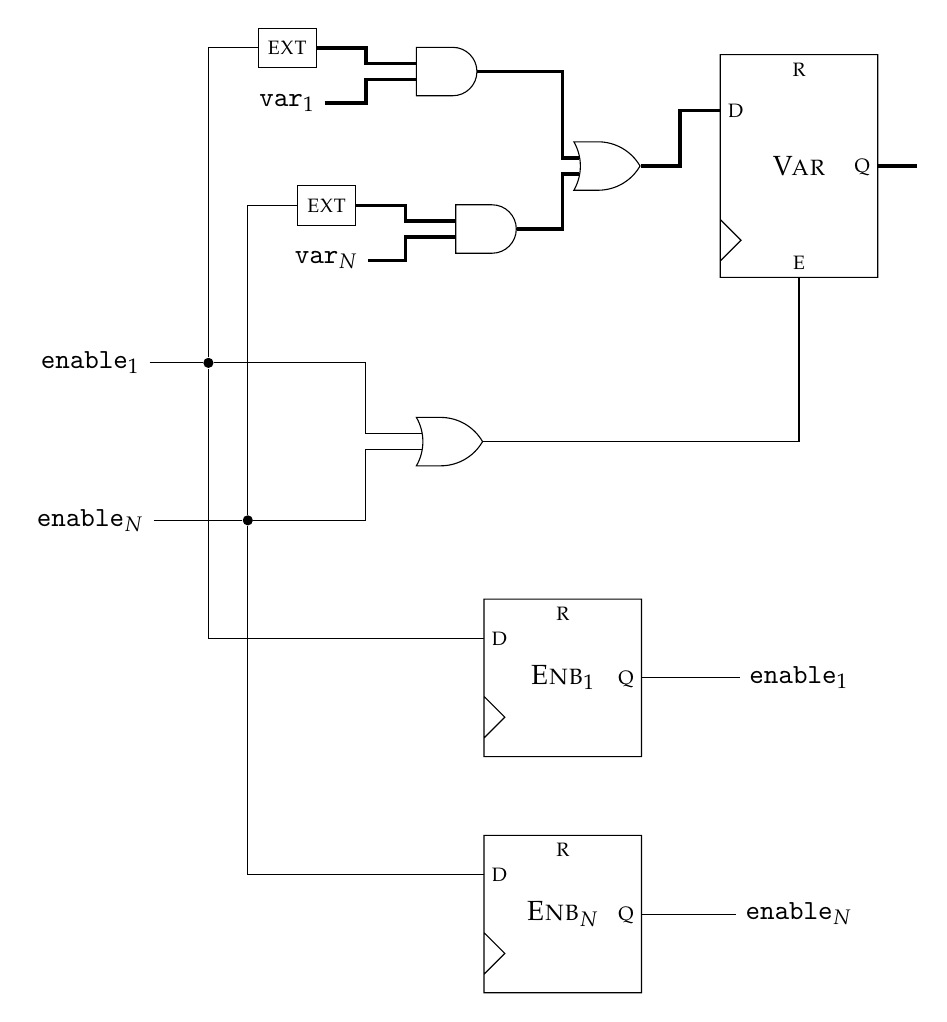
\begin{tikzpicture}[circuit logic US,%
        dot/.style    = {anchor=base,fill,circle,inner sep=1.3pt}]

\node at (-1,1) (e1) {$\texttt{enable}_1$};
\node at (-1,-1) (en) {$\texttt{enable}_N$};
\node at (1.5,4.3) (x1) {$\texttt{var}_1$};
\node at (2,2.3) (xn) {$\texttt{var}_N$};
\node[dot] at (0.5,1) (aux_e1) {};
\node[dot] at (1,-1) (aux_en) {};
\node[draw,rectangle,minimum width=0.5cm,minimum height=0.5cm] at (1.5,5) (ext1) {\scriptsize \textsc{EXT}};
\node[draw,rectangle,minimum width=0.5cm,minimum height=0.5cm] at (2,3) (extn) {\scriptsize \textsc{EXT}};
\node[and gate,inputs=nn] at (3.5,4.7) (and_x1) {};
\node[and gate,inputs=nn] at (4,2.7) (and_xn) {};
\node[or gate,inputs=nn] at (5.5,3.5) (or_x) {};
\node[or gate,inputs=nn] at (3.5,0) (or_enb) {};
\node[shape=dff] at (8,3.5) (ff_x) {\textsc{Var}};
\node[shape=dffne] at (5,-3) (ff_e1) {$\textsc{Enb}_1$};
\node[shape=dffne] at (5,-6) (ff_en) {$\textsc{Enb}_N$};
\node at ($ (ff_e1.Q) + (2,0) $) (e1_out) {$\texttt{enable}_1$};
\node at ($ (ff_en.Q) + (2,0) $) (en_out) {$\texttt{enable}_N$};

\draw (e1.east) -- (aux_e1) |- (ext1.west);
\draw (en.east) -- (aux_en) |- (extn.west);
\draw[very thick] (ext1.east) -- (2.5,5) |- (and_x1.input 1);
\draw[very thick] (x1.east) -- (2.5,4.3) |- (and_x1.input 2);
\draw[very thick] (extn.east) -- (3,3) |- (and_xn.input 1);
\draw[very thick] (xn.east) -- (3,2.3) |- (and_xn.input 2);
\draw[very thick] (and_x1.output) -- (5,4.7) |- (or_x.input 1);
\draw[very thick] (and_xn.output) -- (5,2.7) |- (or_x.input 2);
\draw[very thick] (or_x.output) -- ++(0.5,0) |- (ff_x.D);
\draw[very thick] (ff_x.Q) -- ++(0.5,0);
\draw (aux_e1) -- ++(2,0) |- (or_enb.input 1);
\draw (aux_en) -- ++(1.5,0) |- (or_enb.input 2);
\draw (or_enb.output) -| (ff_x.E);
\draw (aux_e1) |- (ff_e1.D);
\draw (aux_en) |- (ff_en.D);
\draw (ff_e1.Q) -- (e1_out.west);
\draw (ff_en.Q) -- (en_out.west);


\end{tikzpicture}

\end{document}




    \caption{Circuit generat per a una variable amb \(N\) assignacions 
        (en el diagrama, per simplicitat, \(N=2\)).}
    \label{fig:assign}
\end{figure}

La \autoref{fig:assign} mostra el circuit utilitzat per a definir una variable 
a la qual s'assigna algun valor en \(N\) punts diferents del 
programa (aquí, entenem variable en un sentit ampli: un paràmetre d'una funció 
es tracta de la mateixa manera que una variable i, en aquest cas, en les 
crides a una funció es fa una assignació per cadascun dels arguments). Per a 
emmagatzemar el valor de la variable, s'utilitza un biestable \textsc{Var} amb 
senyal d'activació. El biestable ha de canviar de valor cada vegada que es 
realitza alguna de les assignacions, de manera que el senyal d'activació 
\textsc{e} d'aquest està connectat a la sortida d'una porta \textit{or} 
que té per entrades tots els senyals d'activació de les assignacions. En 
aquest cas, el senyal d'entrada \textsc{d} ha de filtrar el valor corresponent 
a l'assignació que s'està executant. Per fer-ho, es repliquen els senyals 
d'activació fins a obtenir busos de \(n\) bits i aquests s'utilitzen com a 
entrades de portes \textit{and} juntament amb els valors a assignar (així 
que la sortida de la porta corresponent a l'assignació en execució és el valor 
a assignar i les sortides de totes les altres portes són 0); finalment, les 
sortides d'aquestes portes \textit{and} s'utilitzen com a entrada d'una porta 
\textit{or} de la qual s'obté el valor a assignar. D'altra banda, una 
assignació tarda un cicle de rellotge a tenir lloc i, per tant, cal retardar 
un cicle la propagació dels senyals d'activació de les assignacions a 
\textsc{Var} mitjançant biestables \(\textsc{Enb}_1,\ldots,\textsc{Enb}_N\)
sense senyal d'activació.

\begin{figure}[ht]
    \centering
    \documentclass[tikz,12pt,border=12pt]{standalone}

\usepackage{mathpazo}
\usepackage[scaled=1.03,varqu]{zi4}
\usepackage[T1]{fontenc}
\usepackage[utf8]{inputenc}
\usepackage{mathtools}
\usepackage{pgf,tikz}
\usetikzlibrary{circuits.logic.US}


%%%%%%%%%%%%%%%%%%%%%%%%%%%%%%%%%%%%%%%%%%%%%%%%%%%%%%%%%%%%%%%%%%%%%%%%%%%%%%%

\makeatletter

% Data Flip Flip (DFF) shape
\pgfdeclareshape{dff}{
  % The 'minimum width' and 'minimum height' keys, not the content, determine
  % the size
  \savedanchor\northeast{%
    \pgfmathsetlength\pgf@x{\pgfshapeminwidth}%
    \pgfmathsetlength\pgf@y{\pgfshapeminheight}%
    \pgf@x=0.5\pgf@x
    \pgf@y=0.5\pgf@y
  }
  % This is redundant, but makes some things easier:
  \savedanchor\southwest{%
    \pgfmathsetlength\pgf@x{\pgfshapeminwidth}%
    \pgfmathsetlength\pgf@y{\pgfshapeminheight}%
    \pgf@x=-0.5\pgf@x
    \pgf@y=-0.5\pgf@y
  }
  % Inherit from rectangle
  \inheritanchorborder[from=rectangle]

  % Define same anchor a normal rectangle has
  \anchor{center}{\pgfpointorigin}
  \anchor{north}{\northeast \pgf@x=0pt}
  \anchor{east}{\northeast \pgf@y=0pt}
  \anchor{south}{\southwest \pgf@x=0pt}
  \anchor{west}{\southwest \pgf@y=0pt}
  \anchor{north east}{\northeast}
  \anchor{north west}{\northeast \pgf@x=-\pgf@x}
  \anchor{south west}{\southwest}
  \anchor{south east}{\southwest \pgf@x=-\pgf@x}
  \anchor{text}{
    \pgfpointorigin
    \advance\pgf@x by -.5\wd\pgfnodeparttextbox%
    \advance\pgf@y by -.5\ht\pgfnodeparttextbox%
    \advance\pgf@y by +.5\dp\pgfnodeparttextbox%
  }

  % Define anchors for signal ports
  \anchor{D}{
    \pgf@process{\northeast}%
    \pgf@x=-1\pgf@x%
    \pgf@y=.5\pgf@y%
  }
  \anchor{CLK}{
    \pgf@process{\northeast}%
    \pgf@x=-1\pgf@x%
    \pgf@y=-.66666\pgf@y%
  }
  \anchor{Q}{
    \pgf@process{\northeast}%
    \pgf@y=0pt%
  }
  \anchor{R}{
    \pgf@process{\northeast}%
    \pgf@x=0pt%
  }
  \anchor{E}{
    \pgf@process{\northeast}%
    \pgf@x=0pt%
    \pgf@y=-\pgf@y%
  }
  % Draw the rectangle box and the port labels
  \backgroundpath{
    % Rectangle box
    \pgfpathrectanglecorners{\southwest}{\northeast}
    % Angle (>) for clock input
    \pgf@anchor@dff@CLK
    \pgf@xa=\pgf@x \pgf@ya=\pgf@y
    \pgf@xb=\pgf@x \pgf@yb=\pgf@y
    \pgf@xc=\pgf@x \pgf@yc=\pgf@y
    \pgfmathsetlength\pgf@x{1.6ex} % size depends on font size
    \advance\pgf@ya by \pgf@x
    \advance\pgf@xb by \pgf@x
    \advance\pgf@yc by -\pgf@x
    \pgfpathmoveto{\pgfpoint{\pgf@xa}{\pgf@ya}}
    \pgfpathlineto{\pgfpoint{\pgf@xb}{\pgf@yb}}
    \pgfpathlineto{\pgfpoint{\pgf@xc}{\pgf@yc}}
    \pgfclosepath

    % Draw port labels
    \begingroup
    \tikzset{flip flop/port labels} % Use font from this style
    \tikz@textfont

    \pgf@anchor@dff@D
    \pgftext[left,base,at={\pgfpoint{\pgf@x}{\pgf@y}},x=\pgfshapeinnerxsep]{\raisebox{-0.75ex}{D}}

    \pgf@anchor@dff@Q
    \pgftext[right,base,at={\pgfpoint{\pgf@x}{\pgf@y}},x=-\pgfshapeinnerxsep]{\raisebox{-.75ex}{Q}}

    \pgf@anchor@dff@R
    \pgftext[top,at={\pgfpoint{\pgf@x}{\pgf@y}},y=-\pgfshapeinnerysep]{R}

    \pgf@anchor@dff@E
    \pgftext[bottom,at={\pgfpoint{\pgf@x}{\pgf@y}},y=\pgfshapeinnerysep]{E}
    \endgroup
  }
}

% Key to add font macros to the current font
\tikzset{add font/.code={\expandafter\def\expandafter\tikz@textfont\expandafter{\tikz@textfont#1}}} 

% Define default style for this node
\tikzset{flip flop/port labels/.style={font=\rmfamily\scriptsize}}
\tikzset{every dff node/.style={draw,minimum width=2cm,minimum 
height=2.828427125cm,inner sep=1mm,outer sep=0pt,cap=round,add 
font=\rmfamily}}

\makeatother

%%%%%%%%%%%%%%%%%%%%%%%%%%%%%%%%%%%%%%%%%%%%%%%%%%%%%%%%%%%%%%%%%%%%%%%%%%%%%%%
%%%%%%%%%%%%%%%%%%%%%%%%%%%%%%%%%%%%%%%%%%%%%%%%%%%%%%%%%%%%%%%%%%%%%%%%%%%%%%%

\makeatletter

% Data Flip Flip (DFF) shape
\pgfdeclareshape{dffne}{
  % The 'minimum width' and 'minimum height' keys, not the content, determine
  % the size
  \savedanchor\northeast{%
    \pgfmathsetlength\pgf@x{\pgfshapeminwidth}%
    \pgfmathsetlength\pgf@y{\pgfshapeminheight}%
    \pgf@x=0.5\pgf@x
    \pgf@y=0.5\pgf@y
  }
  % This is redundant, but makes some things easier:
  \savedanchor\southwest{%
    \pgfmathsetlength\pgf@x{\pgfshapeminwidth}%
    \pgfmathsetlength\pgf@y{\pgfshapeminheight}%
    \pgf@x=-0.5\pgf@x
    \pgf@y=-0.5\pgf@y
  }
  % Inherit from rectangle
  \inheritanchorborder[from=rectangle]

  % Define same anchor a normal rectangle has
  \anchor{center}{\pgfpointorigin}
  \anchor{north}{\northeast \pgf@x=0pt}
  \anchor{east}{\northeast \pgf@y=0pt}
  \anchor{south}{\southwest \pgf@x=0pt}
  \anchor{west}{\southwest \pgf@y=0pt}
  \anchor{north east}{\northeast}
  \anchor{north west}{\northeast \pgf@x=-\pgf@x}
  \anchor{south west}{\southwest}
  \anchor{south east}{\southwest \pgf@x=-\pgf@x}
  \anchor{text}{
    \pgfpointorigin
    \advance\pgf@x by -.5\wd\pgfnodeparttextbox%
    \advance\pgf@y by -.5\ht\pgfnodeparttextbox%
    \advance\pgf@y by +.5\dp\pgfnodeparttextbox%
  }

  % Define anchors for signal ports
  \anchor{D}{
    \pgf@process{\northeast}%
    \pgf@x=-1\pgf@x%
    \pgf@y=.5\pgf@y%
  }
  \anchor{CLK}{
    \pgf@process{\northeast}%
    \pgf@x=-1\pgf@x%
    \pgf@y=-.5\pgf@y%
  }
  \anchor{Q}{
    \pgf@process{\northeast}%
    \pgf@y=0pt%
  }
  \anchor{R}{
    \pgf@process{\northeast}%
    \pgf@x=0pt%
  }
  % Draw the rectangle box and the port labels
  \backgroundpath{
    % Rectangle box
    \pgfpathrectanglecorners{\southwest}{\northeast}
    % Angle (>) for clock input
    \pgf@anchor@dffne@CLK
    \pgf@xa=\pgf@x \pgf@ya=\pgf@y
    \pgf@xb=\pgf@x \pgf@yb=\pgf@y
    \pgf@xc=\pgf@x \pgf@yc=\pgf@y
    \pgfmathsetlength\pgf@x{1.6ex} % size depends on font size
    \advance\pgf@ya by \pgf@x
    \advance\pgf@xb by \pgf@x
    \advance\pgf@yc by -\pgf@x
    \pgfpathmoveto{\pgfpoint{\pgf@xa}{\pgf@ya}}
    \pgfpathlineto{\pgfpoint{\pgf@xb}{\pgf@yb}}
    \pgfpathlineto{\pgfpoint{\pgf@xc}{\pgf@yc}}
    \pgfclosepath

    % Draw port labels
    \begingroup
    \tikzset{flip flop/port labels} % Use font from this style
    \tikz@textfont

    \pgf@anchor@dffne@D
    \pgftext[left,base,at={\pgfpoint{\pgf@x}{\pgf@y}},x=\pgfshapeinnerxsep]{\raisebox{-0.75ex}{D}}

    \pgf@anchor@dffne@Q
    \pgftext[right,base,at={\pgfpoint{\pgf@x}{\pgf@y}},x=-\pgfshapeinnerxsep]{\raisebox{-.75ex}{Q}}

    \pgf@anchor@dffne@R
    \pgftext[top,at={\pgfpoint{\pgf@x}{\pgf@y}},y=-\pgfshapeinnerysep]{R}
    \endgroup
  }
}

% Key to add font macros to the current font
%\tikzset{add font/.code={\expandafter\def\expandafter\tikz@textfont\expandafter{\tikz@textfont#1}}} 

% Define default style for this node
%\tikzset{flip flop/port labels/.style={font=\rmfamily\scriptsize}}
\tikzset{every dffne node/.style={draw,minimum width=2cm,minimum 
height=2cm,inner sep=1mm,outer sep=0pt,cap=round,add 
font=\rmfamily}}

\makeatother

%%%%%%%%%%%%%%%%%%%%%%%%%%%%%%%%%%%%%%%%%%%%%%%%%%%%%%%%%%%%%%%%%%%%%%%%%%%%%%%


\begin{document}

\begin{tikzpicture}[circuit logic US,%
        dot/.style    = {anchor=base,fill,circle,inner sep=1.3pt}]

\node at (-2,1) (e1) {$\texttt{enable}_1$};
\node at (-2,-1) (en) {$\texttt{enable}_N$};
\node[or gate,inputs=nn] at (1,0) (or_enb) {};
\node[dot] at (2,0) (aux_enb_in) {};
\node[dot] at (0,1) (aux_e1) {};
\node[dot] at (-0.5,-1) (aux_en) {};
\node[draw,rectangle,minimum width=3cm,minimum height=3cm] at (5,0.75) (f) {\textsc{Func}};
\node[and gate,inputs=nn] at (3,-2) (and1t) {};
\node[and gate,inputs=in] at (3,-3) (and1f) {};
\node[and gate,inputs=nn] at (3,-7) (andnt) {};
\node[and gate,inputs=in] at (3,-8) (andnf) {};
\node[dot] at (2,-1.9) (aux1_enb) {};
\node[dot] at (2,-2.9) (aux2_enb) {};
\node[dot] at (2,-6.9) (aux3_enb) {};
\node[or gate,inputs=nn] at (4.5,-2.5) (or1) {};
\node[or gate,inputs=nn] at (4.5,-7.5) (orn) {};
\node[shape=dffne] at (6.5,-3) (rege1) {$\textsc{Enb}_1$};
\node[shape=dffne] at (6.5,-8) (regen) {$\textsc{Enb}_N$};
\node[dot] at (8,-3) (aux1_out) {};
\node[dot] at (8,-8) (aux2_out) {};
\node[and gate] at (9.5,-2.5) (and1_out) {};
\node[and gate] at (9,-7.5) (andn_out) {};
\node[dot] at (8.5,0) (aux_out) {};
\node at (11,-2.5) (e1_) {$\texttt{enable}_1$};
\node at (11,-7.5) (en_) {$\texttt{enable}_N$};

\draw (e1.east) -- (0.5,1) |- (or_enb.input 1);
\draw (en.east) -- (0.5,-1) |- (or_enb.input 2);
\draw (or_enb.output) -- (aux_enb_in) -- ($ (f.west) + (0,-0.75) $); 
\draw (aux_e1) |- (and1t.input 2);
\draw (aux_en) |- (andnt.input 2);
\draw (aux1_enb) -- (and1t.input 1);
\draw (aux2_enb) -- (and1f.input 1);
\draw (aux3_enb) -- (andnt.input 1);
\draw (aux_enb_in) |- (andnf.input 1);
\draw (and1t.output) -- ++(0.5,0) |- (or1.input 1);
\draw (and1f.output) -- ++(0.5,0) |- (or1.input 2);
\draw (andnt.output) -- ++(0.5,0) |- (orn.input 1);
\draw (andnf.output) -- ++(0.5,0) |- (orn.input 2);
\draw (or1.output) -- (rege1.D);
\draw (orn.output) -- (regen.D);
\draw (aux1_out) -- ++(0,-1.5) -- ++(-5.5,0) |- (and1f.input 2);
\draw (aux2_out) -- ++(0,-1.5) -- ++(-5.5,0) |- (andnf.input 2);
\draw (rege1.Q) -- ++(1.5,0) |- (and1_out.input 2);
\draw (regen.Q) -- ++(1,0) |- (andn_out.input 2);
\draw (6.5,0) -- ++(2.5,0) |- (and1_out.input 1);
\draw (aux_out) |- (andn_out.input 1);
\draw (and1_out.output) -- (e1_.west);
\draw (andn_out.output) -- (en_.west);

\end{tikzpicture}

\end{document}




    \caption{Circuit generat per a una funció amb \(N\) crides 
        (en el diagrama, per simplicitat, \(N=2\)).}
    \label{fig:func}
\end{figure}

Per a definir una funció tenint en compte les crides que s'hi fan també cal 
construir un circuit similar, tal com s'observa a la \autoref{fig:func}. En 
particular, en aquest diagrama es considera una funció a la qual es fan crides
en \(N\) punts diferents del programa. Primer de tot, es tradueix 
recursivament el cos de la funció per generar el circuit \textsc{Func}. 
Aquest s'ha d'activar quan hi hagi alguna crida a la funció; és a dir, el 
senyal d'activació d'entrada és el resultat d'una porta \textit{or} amb 
entrades els senyals d'activació de cadascuna de les crides. Ara bé, en 
acabar l'execució de la funció, cal saber quina crida s'estava executant per 
poder retornar al punt del programa adequat. Per aconseguir-ho, per a cada 
crida es col·loca un biestable sense senyal d'activació juntament amb un 
circuit que permet emmagatzemar el valor del senyal d'activació d'entrada 
durant l'execució de la funció. Concretament, per a cada crida donada, 
s'utilitzen dues portes \textit{and}: una amb entrades el senyal d'activació 
d'entrada del cos de la funció i el senyal d'activació de la crida (així se 
sap si aquella crida s'ha activat), i una altra amb entrades el senyal 
d'activació d'entrada del cos de la funció negat i el senyal \textsc{q} del 
biestable corresponent (així es manté el valor previ mentre s'executa la 
funció). Les sortides d'aquestes dues es combinen amb una porta \textit{or} i 
el resultat d'aquesta es connecta al senyal \textsc{d} del biestable (és a dir, 
quan comença una crida, el biestable corresponent a la crida pren el valor 1 
i tots els altres biestables prenen el valor 0, i aquests valors es mantenen 
durant tota l'execució de la funció i, de fet, fins a la següent crida). 
Finalment, els senyals d'activació de sortida es calculen amb una porta 
\textit{and} amb entrades el senyal \textsc{q} del biestable corresponent i 
el senyal d'activació de sortida del cos de la funció (d'aquesta manera, quan 
l'execució del cos de la funció acaba, es retorna al punt on s'ha cridat i no 
a cap altre). Com que l'execució d'una funció triga almenys un cicle de 
rellotge (per l'assignació final obligatòria), aquest circuit funciona 
correctament. 

Les crides a funcions es redueixen als dos casos anteriors. És a dir, una 
crida es descompon en dues parts: en la primera, els arguments s'assignen 
seqüencialment a les variables de la funció cridada que actuen com a 
paràmetres (per tant, tan sols cal connectar els valors dels arguments i els 
senyals d'activació al circuit explicat per a les assignacions); en la segona, 
s'activa l'execució de la funció cridada (per tant, tan sols cal connectar 
els senyals d'activació al circuit explicat per a la definició de funcions). 
Per utilitzar el valor retornat per la crida, tan sols cal utilitzar la 
variable especial amb el mateix nom de la funció (o sigui, es pot connectar 
directament el senyal \textsc{q} del biestable que emmagatzema aquesta 
variable al circuit del càlcul de l'expressió on s'ha fet la crida).

Ara que s'ha descrit formalment el mètode de generació de circuits, passem a 
comentar breument alguns detalls particulars del programa que s'encarrega de 
fer-ho. Aquest parteix des de l'arrel de l'AST i, per a cada funció, genera 
el circuit corresponent a totes les variables (incloent paràmetres i la 
variable especial de retorn) d'aquesta i llavors genera el circuit que 
controla les crides a aquesta funció. Seguidament, es tradueix recursivament 
el cos de la funció segons les regles explicades i seguint els nodes de 
l'arbre. Per connectar correctament els diferents components, quan s'accedeix 
a una funció es coneixen el nombre de crides i el nombre d'assignacions a 
cadascuna de les seves variables (gràcies al procés explicat en la 
\autoref{sec:graf}); així, es poden generar tants cables per a les 
assignacions a variables i les crides a la funció com faci falta. D'altra 
banda, quan, en la traducció del cos d'una funció, s'arriba a una assignació o 
a una crida, es disposa d'un identificador numèric que permet associar-lo 
unívocament a un dels cables definits prèviament.

Llevat d'alguns punts més importants del circuit (com ara els descrits), la 
majoria de cables es defineixen en el codi en \texttt{Verilog} amb noms 
formats per un nombre per evitar repeticions (però no tenen un significat 
explicatiu). El motiu és que, en la generació automàtica de circuits, per a 
cada instrucció del codi original cal definir una multitud de variables en 
\texttt{Verilog}.

El programa que hem desenvolupat, doncs, segueix el mètode descrit per generar 
un mòdul en \texttt{Verilog} amb paràmetres d'entrada el senyal de rellotge, 
un senyal de reinici dels biestables (connectat al seu port \textsc{r}) i 
el senyal d'activació d'entrada i paràmetres de sortida el senyal d'activació 
de sortida i el resultat de la funció \texttt{main}. Per tant, es pot simular 
amb alguna eina com \texttt{Icarus Verilog} creant un \textit{testbench} en 
què es generi un senyal de rellotge i s'instanciï el mòdul generat. Cal posar 
el senyal de reinici a 1 durant un cicle al principi i, un cop posats a 0 
tots els biestables, activar l'execució posant a 1 el senyal d'activació 
durant un cicle. El flanc ascendent en el senyal d'activació de sortida 
indica que l'execució ha finalitzat correctament i es disposa del resultat.




\clearpage


\section{Distribució del treball}
Cal mencionar que la part lèxico-sintàctica s'ha dissenyat, desenvolupat i depurat entre els dos integrants del grup. És per aquest motiu que aquesta part (la qual correspondria al primer mòdul dels presentats) no apareix a la repartició de feina que presentem a continuació:

\begin{itemize}
\item Sergio Rodríguez: Part semàntica, generació del graf de crides. Aquesta part correspondria al segon mòdul dels enumerats anteriorment.
\item Francesc Gispert: Generació del \textit{hardware} a partir del codi. És a dir, el tercer i últim mòdul llistat.
\end{itemize}

També es vol fer notar que aquesta repartició de feina és només orientativa i pot variar a la pràctica. 
En particular, aquesta distribució només reflecteix qui assumirà més 
responsabilitats en cadascun dels dos mòduls restants, però els dos integrants 
del grup col·laborarem activament en tot el desenvolupament del projecte.



\clearpage


\section{Gramàtica del llenguatge}

Tot seguit es mostra la gramàtica del llenguatge dissenyat, utilitzant ja el 
llenguatge \texttt{ANTLR} per a descriure-la.

\lstinputlisting%
  [caption={Gramàtica del llenguatge.},style=antlr-gram,label={lst:gramatica}]%
  {../src/parser/hw_compilation.g}



\clearpage


\section{Exemples d'ús}

Finalment, segueixen alguns exemples no trivials d'ús del llenguatge. En 
particular, al \autoref{lst:ex-enters} es mostren alguns algorismes 
elementals utilitzats en teoria de nombres, mentre que al 
\autoref{lst:ex-xifrat} es mostra una estratègia molt simple per xifrar i 
desxifrar blocs de dades. En aquests exemples es poden observar les 
construccions bàsiques que permet el llenguatge.

D'altra banda, amb el codi adjunt a aquest document, s'inclouen exemples que 
realitzen càlculs sense gaire sentit pràctic (o fins i tot incorrectes) i que 
han estat utilitzats durant el desenvolupament del projecte per comprovar el 
correcte funcionament de les diferents funcionalitats implementades.

\lstinputlisting%
  [caption={Exemple d'ús per funcions en enters.},style=hw-comp,label={lst:ex-enters}]%
  {../examples/number_theory.hwc}

\lstinputlisting%
  [caption={Exemple d'ús en un mètode de xifrat.},style=hw-comp,label={lst:ex-xifrat}]%
  {../examples/tea.hwc}




\clearpage

%%%%%%%%%%%%%%%%%%%%%%%%%%%%%%%%%%%%%%%%%%%%%%%%%%%%%%%%%%%%%%%%%%%%%%%%%%%%%%%

\nocite{*}
\printbibliography[heading=bibintoc]

\end{document}
